\section{Kapitel 6}
\subsection{Teilaufgabe 1}
\subsubsection{Aufgabenstellung}
Im grunde ist es die Selbe Aufgabe wie aus Kapitel 4, Teilaufgabe 2. Doch jetzt solle es auch
für nxn Matrizen funktionieren. Die grö\ss\space gibt an ende der Nutzer ein. Zusätzlich soll
noch die Multiplikation der Matrizen auch mit while und do-while gelöst werden.

\subsubsection{Anforderungsdefinition}
\begin{enumerate}
	\item Unser input für die Grö\ss\space der nxn Matrix.
	\item Multiplikation mit for, while, und do-while.
\end{enumerate}

\subsubsection{Entwurf}
% generated by Plantuml 1.2018.13      
\definecolor{plantucolor0000}{RGB}{0,0,0}
\definecolor{plantucolor0001}{RGB}{254,254,206}
\definecolor{plantucolor0002}{RGB}{168,0,54}
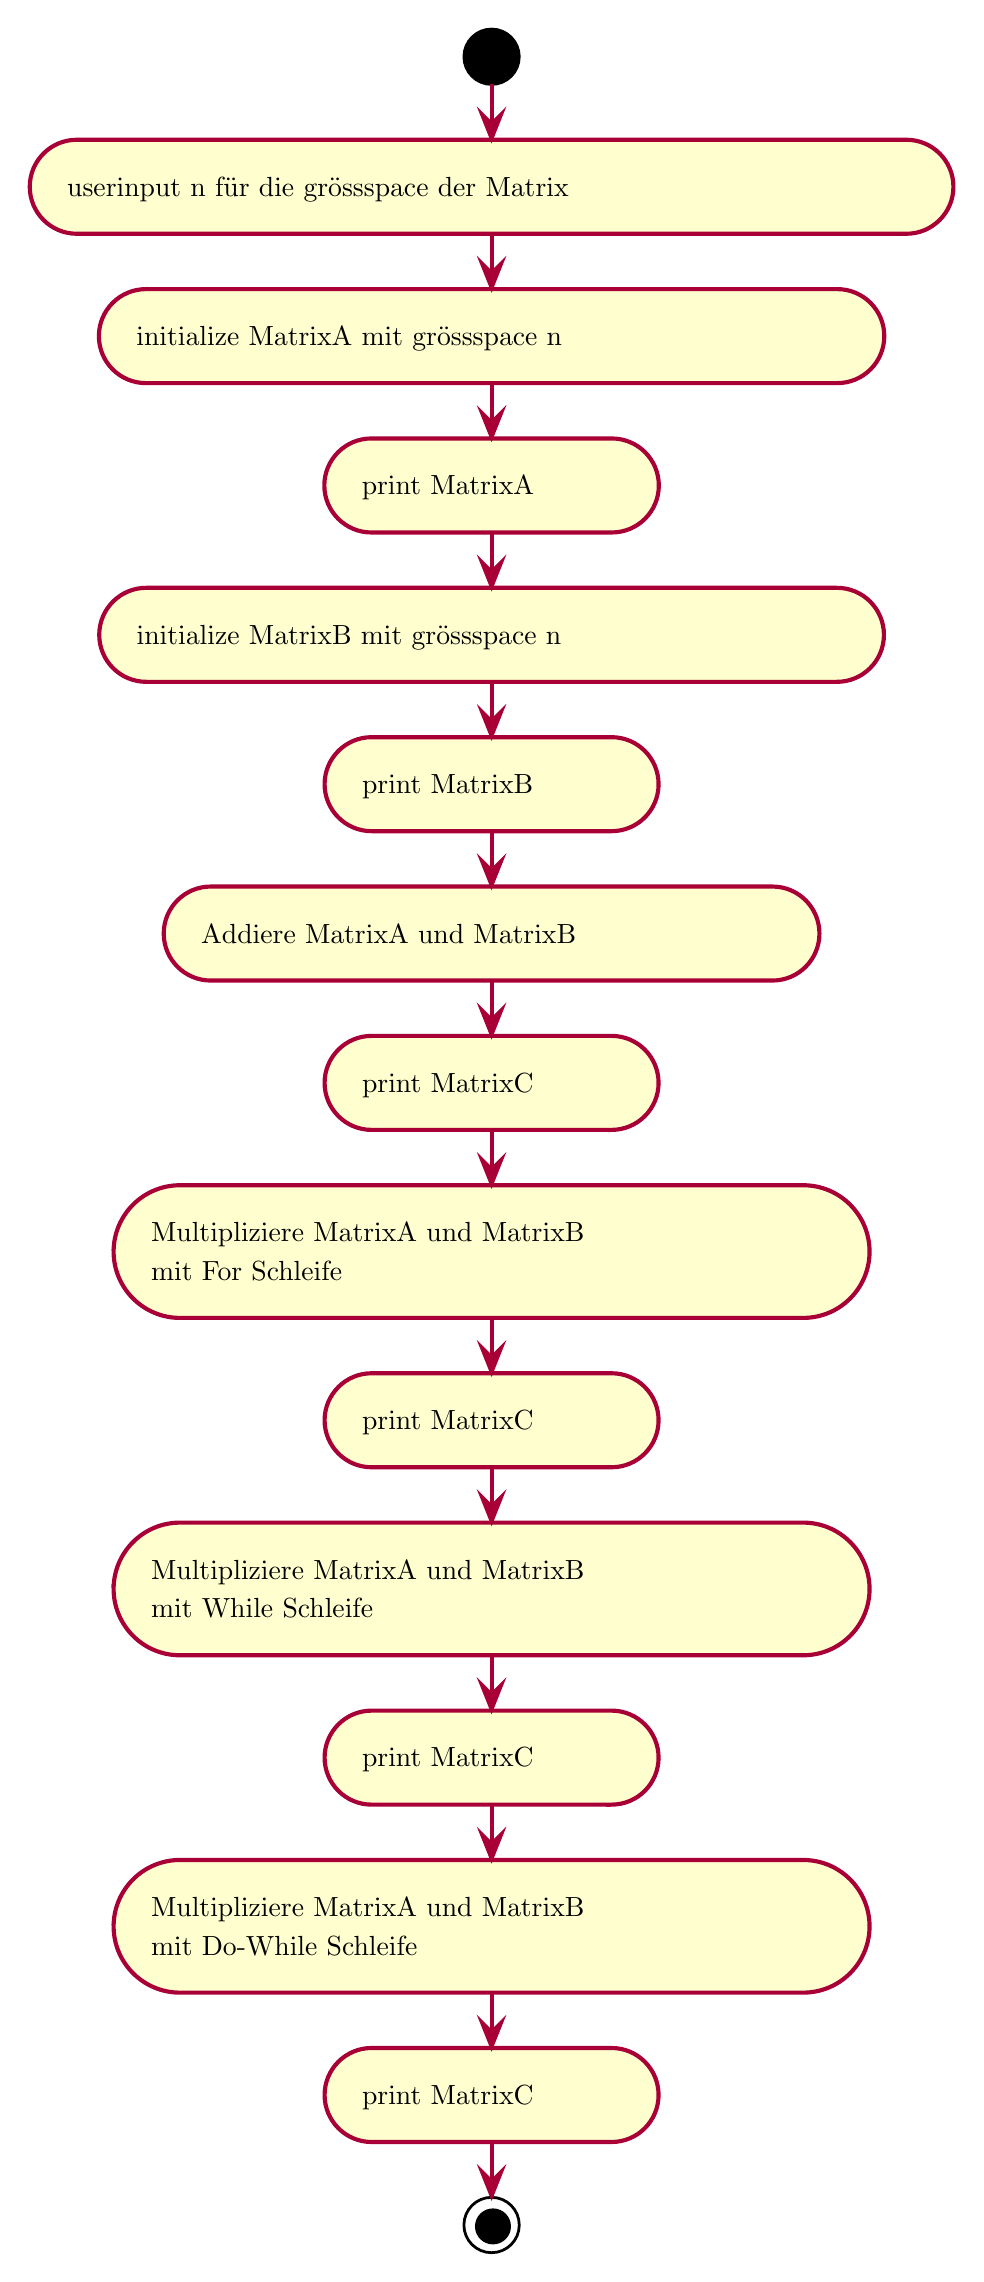
\begin{tikzpicture}[yscale=-1
,pstyle0/.style={fill=black,line width=1.0pt}
,pstyle1/.style={color=plantucolor0002,fill=plantucolor0001,line width=1.5pt}
,pstyle3/.style={color=plantucolor0002,line width=1.5pt}
,pstyle4/.style={color=plantucolor0002,fill=plantucolor0002,line width=1.0pt}
]
\draw[pstyle0] (176.8821pt,20pt) ellipse (10pt and 10pt);
\draw[pstyle1] (10pt,66.9844pt) arc (180:270:16.9844pt) -- (26.9844pt,50pt) -- (326.7798pt,50pt) arc (270:360:16.9844pt) -- (343.7642pt,66.9844pt) -- (343.7642pt,66.9844pt) arc (0:90:16.9844pt) -- (326.7798pt,83.9688pt) -- (26.9844pt,83.9688pt) arc (90:180:16.9844pt) -- (10pt,66.9844pt) -- cycle;
\node at (20pt,60pt)[below right,color=black]{userinput n für die grö\\ss\\space der Matrix};
\draw[pstyle1] (34.9821pt,120.9531pt) arc (180:270:16.9844pt) -- (51.9665pt,103.9688pt) -- (301.7977pt,103.9688pt) arc (270:360:16.9844pt) -- (318.7821pt,120.9531pt) -- (318.7821pt,120.9531pt) arc (0:90:16.9844pt) -- (301.7977pt,137.9375pt) -- (51.9665pt,137.9375pt) arc (90:180:16.9844pt) -- (34.9821pt,120.9531pt) -- cycle;
\node at (44.9821pt,113.9688pt)[below right,color=black]{initialize MatrixA mit grö\\ss\\space n};
\draw[pstyle1] (116.4468pt,174.9219pt) arc (180:270:16.9844pt) -- (133.4312pt,157.9375pt) -- (220.333pt,157.9375pt) arc (270:360:16.9844pt) -- (237.3174pt,174.9219pt) -- (237.3174pt,174.9219pt) arc (0:90:16.9844pt) -- (220.333pt,191.9063pt) -- (133.4312pt,191.9063pt) arc (90:180:16.9844pt) -- (116.4468pt,174.9219pt) -- cycle;
\node at (126.4468pt,167.9375pt)[below right,color=black]{print MatrixA};
\draw[pstyle1] (35.1071pt,228.8906pt) arc (180:270:16.9844pt) -- (52.0915pt,211.9063pt) -- (301.6727pt,211.9063pt) arc (270:360:16.9844pt) -- (318.6571pt,228.8906pt) -- (318.6571pt,228.8906pt) arc (0:90:16.9844pt) -- (301.6727pt,245.875pt) -- (52.0915pt,245.875pt) arc (90:180:16.9844pt) -- (35.1071pt,228.8906pt) -- cycle;
\node at (45.1071pt,221.9063pt)[below right,color=black]{initialize MatrixB mit grö\\ss\\space n};
\draw[pstyle1] (116.5409pt,282.8594pt) arc (180:270:16.9844pt) -- (133.5253pt,265.875pt) -- (220.2389pt,265.875pt) arc (270:360:16.9844pt) -- (237.2233pt,282.8594pt) -- (237.2233pt,282.8594pt) arc (0:90:16.9844pt) -- (220.2389pt,299.8438pt) -- (133.5253pt,299.8438pt) arc (90:180:16.9844pt) -- (116.5409pt,282.8594pt) -- cycle;
\node at (126.5409pt,275.875pt)[below right,color=black]{print MatrixB};
\draw[pstyle1] (58.4118pt,336.8281pt) arc (180:270:16.9844pt) -- (75.3962pt,319.8438pt) -- (278.368pt,319.8438pt) arc (270:360:16.9844pt) -- (295.3524pt,336.8281pt) -- (295.3524pt,336.8281pt) arc (0:90:16.9844pt) -- (278.368pt,353.8125pt) -- (75.3962pt,353.8125pt) arc (90:180:16.9844pt) -- (58.4118pt,336.8281pt) -- cycle;
\node at (68.4118pt,329.8438pt)[below right,color=black]{Addiere MatrixA und MatrixB};
\draw[pstyle1] (116.5409pt,390.7969pt) arc (180:270:16.9844pt) -- (133.5253pt,373.8125pt) -- (220.2389pt,373.8125pt) arc (270:360:16.9844pt) -- (237.2233pt,390.7969pt) -- (237.2233pt,390.7969pt) arc (0:90:16.9844pt) -- (220.2389pt,407.7813pt) -- (133.5253pt,407.7813pt) arc (90:180:16.9844pt) -- (116.5409pt,390.7969pt) -- cycle;
\node at (126.5409pt,383.8125pt)[below right,color=black]{print MatrixC};
\draw[pstyle1] (40.3007pt,451.75pt) arc (180:270:23.9688pt) -- (64.2694pt,427.7813pt) -- (289.4947pt,427.7813pt) arc (270:360:23.9688pt) -- (313.4635pt,451.75pt) -- (313.4635pt,451.75pt) arc (0:90:23.9688pt) -- (289.4947pt,475.7188pt) -- (64.2694pt,475.7188pt) arc (90:180:23.9688pt) -- (40.3007pt,451.75pt) -- cycle;
\node at (50.3007pt,437.7813pt)[below right,color=black]{Multipliziere MatrixA und MatrixB};
\node at (50.3007pt,451.75pt)[below right,color=black]{mit For Schleife};
\draw[pstyle1] (116.5409pt,512.7031pt) arc (180:270:16.9844pt) -- (133.5253pt,495.7188pt) -- (220.2389pt,495.7188pt) arc (270:360:16.9844pt) -- (237.2233pt,512.7031pt) -- (237.2233pt,512.7031pt) arc (0:90:16.9844pt) -- (220.2389pt,529.6875pt) -- (133.5253pt,529.6875pt) arc (90:180:16.9844pt) -- (116.5409pt,512.7031pt) -- cycle;
\node at (126.5409pt,505.7188pt)[below right,color=black]{print MatrixC};
\draw[pstyle1] (40.3007pt,573.6563pt) arc (180:270:23.9688pt) -- (64.2694pt,549.6875pt) -- (289.4947pt,549.6875pt) arc (270:360:23.9688pt) -- (313.4635pt,573.6563pt) -- (313.4635pt,573.6563pt) arc (0:90:23.9688pt) -- (289.4947pt,597.625pt) -- (64.2694pt,597.625pt) arc (90:180:23.9688pt) -- (40.3007pt,573.6563pt) -- cycle;
\node at (50.3007pt,559.6875pt)[below right,color=black]{Multipliziere MatrixA und MatrixB};
\node at (50.3007pt,573.6563pt)[below right,color=black]{mit While Schleife};
\draw[pstyle1] (116.5409pt,634.6094pt) arc (180:270:16.9844pt) -- (133.5253pt,617.625pt) -- (220.2389pt,617.625pt) arc (270:360:16.9844pt) -- (237.2233pt,634.6094pt) -- (237.2233pt,634.6094pt) arc (0:90:16.9844pt) -- (220.2389pt,651.5938pt) -- (133.5253pt,651.5938pt) arc (90:180:16.9844pt) -- (116.5409pt,634.6094pt) -- cycle;
\node at (126.5409pt,627.625pt)[below right,color=black]{print MatrixC};
\draw[pstyle1] (40.3007pt,695.5625pt) arc (180:270:23.9688pt) -- (64.2694pt,671.5938pt) -- (289.4947pt,671.5938pt) arc (270:360:23.9688pt) -- (313.4635pt,695.5625pt) -- (313.4635pt,695.5625pt) arc (0:90:23.9688pt) -- (289.4947pt,719.5313pt) -- (64.2694pt,719.5313pt) arc (90:180:23.9688pt) -- (40.3007pt,695.5625pt) -- cycle;
\node at (50.3007pt,681.5938pt)[below right,color=black]{Multipliziere MatrixA und MatrixB};
\node at (50.3007pt,695.5625pt)[below right,color=black]{mit Do-While Schleife};
\draw[pstyle1] (116.5409pt,756.5156pt) arc (180:270:16.9844pt) -- (133.5253pt,739.5313pt) -- (220.2389pt,739.5313pt) arc (270:360:16.9844pt) -- (237.2233pt,756.5156pt) -- (237.2233pt,756.5156pt) arc (0:90:16.9844pt) -- (220.2389pt,773.5pt) -- (133.5253pt,773.5pt) arc (90:180:16.9844pt) -- (116.5409pt,756.5156pt) -- cycle;
\node at (126.5409pt,749.5313pt)[below right,color=black]{print MatrixC};
\draw[color=black,line width=1.0pt] (176.8821pt,803.5pt) ellipse (10pt and 10pt);
\draw[pstyle0] (177.3821pt,804pt) ellipse (6pt and 6pt);
\draw[pstyle3] (176.8821pt,30pt) -- (176.8821pt,50pt);
\draw[pstyle4] (172.8821pt,40pt) -- (176.8821pt,50pt) -- (180.8821pt,40pt) -- (176.8821pt,44pt) -- cycle;
\draw[pstyle3] (176.8821pt,83.9688pt) -- (176.8821pt,103.9688pt);
\draw[pstyle4] (172.8821pt,93.9688pt) -- (176.8821pt,103.9688pt) -- (180.8821pt,93.9688pt) -- (176.8821pt,97.9688pt) -- cycle;
\draw[pstyle3] (176.8821pt,137.9375pt) -- (176.8821pt,157.9375pt);
\draw[pstyle4] (172.8821pt,147.9375pt) -- (176.8821pt,157.9375pt) -- (180.8821pt,147.9375pt) -- (176.8821pt,151.9375pt) -- cycle;
\draw[pstyle3] (176.8821pt,191.9063pt) -- (176.8821pt,211.9063pt);
\draw[pstyle4] (172.8821pt,201.9063pt) -- (176.8821pt,211.9063pt) -- (180.8821pt,201.9063pt) -- (176.8821pt,205.9063pt) -- cycle;
\draw[pstyle3] (176.8821pt,245.875pt) -- (176.8821pt,265.875pt);
\draw[pstyle4] (172.8821pt,255.875pt) -- (176.8821pt,265.875pt) -- (180.8821pt,255.875pt) -- (176.8821pt,259.875pt) -- cycle;
\draw[pstyle3] (176.8821pt,299.8438pt) -- (176.8821pt,319.8438pt);
\draw[pstyle4] (172.8821pt,309.8438pt) -- (176.8821pt,319.8438pt) -- (180.8821pt,309.8438pt) -- (176.8821pt,313.8438pt) -- cycle;
\draw[pstyle3] (176.8821pt,353.8125pt) -- (176.8821pt,373.8125pt);
\draw[pstyle4] (172.8821pt,363.8125pt) -- (176.8821pt,373.8125pt) -- (180.8821pt,363.8125pt) -- (176.8821pt,367.8125pt) -- cycle;
\draw[pstyle3] (176.8821pt,407.7813pt) -- (176.8821pt,427.7813pt);
\draw[pstyle4] (172.8821pt,417.7813pt) -- (176.8821pt,427.7813pt) -- (180.8821pt,417.7813pt) -- (176.8821pt,421.7813pt) -- cycle;
\draw[pstyle3] (176.8821pt,475.7188pt) -- (176.8821pt,495.7188pt);
\draw[pstyle4] (172.8821pt,485.7188pt) -- (176.8821pt,495.7188pt) -- (180.8821pt,485.7188pt) -- (176.8821pt,489.7188pt) -- cycle;
\draw[pstyle3] (176.8821pt,529.6875pt) -- (176.8821pt,549.6875pt);
\draw[pstyle4] (172.8821pt,539.6875pt) -- (176.8821pt,549.6875pt) -- (180.8821pt,539.6875pt) -- (176.8821pt,543.6875pt) -- cycle;
\draw[pstyle3] (176.8821pt,597.625pt) -- (176.8821pt,617.625pt);
\draw[pstyle4] (172.8821pt,607.625pt) -- (176.8821pt,617.625pt) -- (180.8821pt,607.625pt) -- (176.8821pt,611.625pt) -- cycle;
\draw[pstyle3] (176.8821pt,651.5938pt) -- (176.8821pt,671.5938pt);
\draw[pstyle4] (172.8821pt,661.5938pt) -- (176.8821pt,671.5938pt) -- (180.8821pt,661.5938pt) -- (176.8821pt,665.5938pt) -- cycle;
\draw[pstyle3] (176.8821pt,719.5313pt) -- (176.8821pt,739.5313pt);
\draw[pstyle4] (172.8821pt,729.5313pt) -- (176.8821pt,739.5313pt) -- (180.8821pt,729.5313pt) -- (176.8821pt,733.5313pt) -- cycle;
\draw[pstyle3] (176.8821pt,773.5pt) -- (176.8821pt,793.5pt);
\draw[pstyle4] (172.8821pt,783.5pt) -- (176.8821pt,793.5pt) -- (180.8821pt,783.5pt) -- (176.8821pt,787.5pt) -- cycle;
\end{tikzpicture}


\subsubsection{Quelltext}
\paragraph{Matrizen.java}\
\lstinputlisting[language = Java , frame = trBL , escapeinside={(*@}{@*)}]{../chapter_06/src/chapter_06/Matrizen.java}

\subsubsection{Testdokumentation}

\subsubsection{Benutzungshinweise}
Nach dem aufrufen des Programmes, wird der nutzer aufgefordert eine Zahl einzugeben.
Diese muss grö\ss er als ein sein.

\subsubsection{Anwendungsbeispiel}
Nach dem man das Programm gestartet hat, sollte folgende Ausgabe erscheinen:
\begin{lstlisting}[frame = trBL , escapeinside={(*@}{@*)}]
[sebastian@laptop bin]$ java Matrizen 
Dieses Programm berechnet eine zufällig erstellte nxn Matrix
Geben sie n an: 5
Matrix A:
56	64	80	51	83	
28	21	53	57	4	
31	65	76	25	17	
23	14	36	38	1	
12	59	78	21	54	

Matrix B:
22	39	22	22	95	
47	51	16	19	73	
91	43	20	42	15	
44	25	72	19	6	
46	7	58	14	18	

Addition von A und B:
78	103	102	73	178	
75	72	69	76	77	
122	108	96	67	32	
67	39	108	57	7	
58	66	136	35	72	

Multiplikation von A und B:
For Schleife
17582	10744	12342	7939	12992	
9118	5895	6348	4380	5402	
12535	8536	6028	5822	9286	
6158	4116	4244	3020	3993	
13543	7734	7412	5816	7715	

While Schleife
17582	10744	12342	7939	12992	
9118	5895	6348	4380	5402	
12535	8536	6028	5822	9286	
6158	4116	4244	3020	3993	
13543	7734	7412	5816	7715	

Do-While Schleife
17582	10744	12342	7939	12992	
9118	5895	6348	4380	5402	
12535	8536	6028	5822	9286	
6158	4116	4244	3020	3993	
13543	7734	7412	5816	7715	
[sebastian@laptop bin]$ 
\end{lstlisting}